\documentclass{bioinfo}
%!TEX TS-program = pdflatex                                                    %
%!TEX encoding = UTF8                                                          %
%!TEX spellcheck = en-US                                                       %
%------------------------------------------------------------------------------%
% to compile use "latexmk --pdf main.tex"                                      %
%------------------------------------------------------------------------------%
% to count words 
% "pdftotext main_nofigs_nocaptions.pdf - | egrep -e '\w\w\w+' | iconv -f ISO-8859-15 -t UTF-8 | wc -w"
% -----------------------------------------------------------------------------%

\usepackage{url}
\usepackage[english]{babel}
\usepackage[utf8]{inputenc}
\usepackage[T1]{fontenc}
%\usepackage[pdftex]{graphicx} 
%\usepackage{graphics}
%\usepackage{hyperref}
\usepackage{float}
\floatplacement{figure}{H}
\usepackage{booktabs}     % nice tables
\usepackage{tabularx}     % even nicer tabular environments 
\usepackage{amsmath}
\usepackage{amsfonts}
\usepackage{amssymb}
%\usepackage{multicol}
\usepackage{listings}
\usepackage{tikz,times}
\usepackage{courier}
\usepackage[scaled]{beramono}

\usepackage{fancyvrb}

\usetikzlibrary{shapes,arrows}
\usetikzlibrary{arrows,positioning}
\usepackage{xcolor}
\usepackage[font=bf]{subfig}
\usepackage[inline]{trackchanges}

%%%%%%% setup track changes "editors"

\addeditor{mw}
\addeditor{lp}
\addeditor{psl}
\addeditor{ld}
\addeditor{sk}
\addeditor{vj}
\addeditor{jm}

\renewcommand{\lstlistingname}{Code}
\renewcommand{\thesubfigure}{\Alph{subfigure}}
%\newcommand{\inputTikZ}[2]{\scalebox{#1}{\input{#2}}}
\newcommand*{\h}{\hspace{5pt}}   % for indentation
\newcommand*{\hh}{\h\h}          % double indentation
\newcommand*{\tvbmodule}[1]{{\textsc{#1}}}          % scientific modules in "simulator"
\newcommand*{\tvbdatatype}[1]{\textbf{\emph{#1}}}   % datatypes in "datatypes"
\newcommand*{\tvbclass}[1]{{\ttfamily\emph{#1}}}    % classes either in simulator mods or datatypes
\newcommand*{\tvbmethod}[1]{{\textsf{#1}}}          % methods
\newcommand*{\tvbattribute}[1]{{\ttfamily{#1}}}     % attributes
\newcommand*{\tvbtrait}[1]{{\ttfamily{#1}}}         % traited types
\newcommand{\TVB}{\textit{TheVirtualBrain }}

\newcommand{\matlab}{MATLAB}

\definecolor{palegreen}{HTML}{DAFFDA}
\definecolor{lightgray}{rgb}{0.15,0.15,0.15}
\definecolor{orange}{HTML}{FF7300}
\DeclareGraphicsExtensions{.jpg,.pdf,.png,.tiff}%,.mps,.bmp
\graphicspath{{figures/}}
 
\copyrightyear{2014}
\pubyear{2014}

\begin{document}
\lstset{language=Python,
	captionpos=b,
	keepspaces=true,
	numbers=none,
	showspaces=false,
    float=*,
	basicstyle=\fontsize{8pt}{8}\ttfamily
	} 

\firstpage{1}

\title[The Virtual Brain]{Integrating neuroinformatics tools in TheVirtualBrain}
\author[Woodman {et~al}]{
        M. Marmaduke Woodman\,$^{1,2,*}$,  
        Laurent Pezard\,$^{1,2}$,  
        Lia Domide\,$^{3}$, 
        Stuart Knock\,$^{1,2}$, 
        Paula Sanz Leon\,$^{1,2}$, 
        Jochen Mersmann\,$^{2}$,
        Anthony R. McIntosh \,$^{4}$ and  
        Viktor Jirsa\,$^{1,,2}$\footnote{to whom correspondence should be addressed: marmaduke.woodman@univ-amu.fr,
        viktor.jirsa@univ-amu.fr}}

\address{$^{1}$ Institut National de la Sant\'{e} et de la Recherche M\'{e}dicale UMR 1106, Institut de Neurosciences des Syst\`{e}mes, 13385 Marseille, France.\\
	 $^{2}$ Aix-Marseille Universit\'{e}, 13284 Marseille, France.\\
         $^{3}$ CodeBox GmbH, Hugo Eckener Str. 7, 70184 Stuttgart, Germany.\\
         $^{4}$ Codemart, 13, Petofi Sandor, 400610, Cluj-Napoca, Romania.\\
         $^{5}$ Rotman Research Institute at Baycrest, Toronto, M6A 2E1, Ontario, Canada\\
        }

\history{}

\editor{}

\maketitle

\begin{abstract}
\section{}

TheVirtualBrain (TVB) is a neuroinformatics Python package representing the
convergence of clinical, systems, and theoretical neuroscience in the analysis,
visualization and modeling of neural and neuroimaging dynamics.  TVB is
composed of a flexible simulator for neural dynamics measured across scales
from local populations to large-scale dynamics measured by
electroencephalography (EEG), magnetoencephalography (MEG) and functional
magnetic resonance imaging (fMRI), and core analytic and visualization
functions, all accessible through a web browser user interface.  A datatype
system modeling neuroscientific data ties together these pieces with persistent
data storage, based on a combination of SQL \& HDF5.  These datatypes combine
with adapters allowing TVB to integrate other algorithms or computational
systems.  TVB provides infrastructure for multiple projects and multiple users,
possibly participating under multiple roles. For example, a clinician might
import patient data to identify several potential lesion points in the
patient's connectome.  A modeler, working on the same project, tests these
points for viability through whole brain simulation, based on the patient's
connectome, and subsequent analysis of dynamical features.  TVB also drives
research forward: the simulator itself represents the culmination of several
simulation frameworks in the modeling literature. The availability of the
numerical methods, set of neural mass models and forward solutions allows for
the construction of a wide range of brain-scale simulation scenarios.  This
paper briefly outlines the history and motivation for TVB, describing the
framework and simulator, giving usage examples in the web UI and Python
scripting.
  
\section{Keywords:} large-scale brain network, simulation, web platform,
Python, connectivity, connectome, neural mass, time delays, functional MRI,
electroencephalography, magnetoencephalography

\end{abstract}

\section{Introduction}

Neuroscience has evolved through extensive interactions among disciplines
to advance our appreciation of the relation between brain and behavior.
The interdisciplinary nature of the field presents formidable challenges
for effective collaboration.

These challenges call for two kinds of solutions. First, there is a need for
comprehensive, modern computational libraries written in widely used and
available programming languages; current examples include MNE-Python
\citep{mnepython}, a Python package for treating M/EEG data via time-frequency
analyses and inverse solutions and the Brain Connectivity Toolbox
\citep{rubinov2010complex} for analyzing the graph theoretic properties of
structural and functional connectivity. Second, there is a need for the
implementation of collaborative infrastructure for sharing not only data, but
expertise; CARMEN \citep{austin2011carmen} and G-Node \citep{herz2008g} are two
such examples of developing platforms for collaborative work and data sharing,
in the domains of cellular and systems neurophysiology.

TheVirtualBrain (TVB) provides new tools to facilitate the collaboration
between experimentalists and modelers by exposing both a comprehensive
simulator for brain dynamics and an integrative framework for the management,
analysis, and simulation of structural and functional data in an accessible,
web-based interface. The choice of Python was made based on its wide use as the
high-level language in scientific programming, the unparalleled open-source
libraries and tools available, and strong software engineering culture.  This
choice was confirmed by the publication of the first issue of Python in
Neuroscience and has made it possible for the entirety of TVB from the
numerical algorithms to the web server to be written in Python.

In the following, we briefly outline the scope of TVB, how to use it before detailing
aspects of the architecture and simulator.

\subsection{Overview}

TVB consists of a framework and a simulator. 
The framework manages projects involving various data, subjects, and users
and the different roles that the users might play in the projects (modeler, 
clinician, etc.). The framework also maintains a database of the different
operations performed by the users in each project as well as the various
data associated with those operations, such as structural and functional
neuroimaging data.
The simulator provides numerical methods to construct and simulate models
based on human cortical and sub-cortical anatomy and dynamics. It employs principally
a neural mass approach, incorporated realistic long-range (delayed) and
short-range connectivity kernels, as well as stochastic fluctuations. 
To make the connection with experimental data, it provides forward solutions to
compute neuroimaging data (fMRI, M/EEG) from the underlying neural dynamics. 
Finally, an graphical interface allows users to take advantage of the framework
and simulator. These components have been described previously by 
\citeauthor{Sanz-Leon_2013} \citeyear{Sanz-Leon_2013} in a general overview
of TVB.

\subsection{Obtaining and using TVB}

The easiest way to get started with TVB is to download a distribution
\footnote{\url{http://www.thevirtualbrain.org}}, which is available for Windows,
Mac OS X and Linux. This distribution includes
all of pieces, from the simulator to the web interface, and has no
requirements other than a modern web browser supporting WebGL, SVG and
HTML5.

Alternatively, because TVB is licensed under the GPL v. 2, the sources may be
readily obtained from the public Git repositories hosted on GitHub \footnote{\url{https://github.com/the-virtual-brain}} 
\citep{dabbish2012social}
. In order to use the simulator, 
only the standard scientific Python packages are required (NumPy \& SciPy).
The framework and web interface depend on a few more packages. 

Documentation including an installation guide, web interface and console 
user guides as well as other information are available online
\footnote{ \url{http://the-virtual-brain.github.io}}.
We provide an API doc, built from the docs strings using Sphinx.
User's, Contributor's and Developer's manuals are also provided with TVB
distributions in PDF format. The source files (in .rst) are available
from the Git repositories.
In addition, IPython notebooks \citep{PerezGranger_2007}
for interactive tutorials are provided. These are based on the
demonstration scripts provided with the scientific library, and
include a more detailed description of the scientific goal (if
applicable), the components and stages of a simulation as well as a
brief description in the case of reproducing previous work. Users
interacting with \TVB GUI may also benefit from these tutorials.
Finally, the user interface provides an online help overlay, that pulls
information from the User's manual.

\section{Architecture}

\begin{figure*}
	\centering
	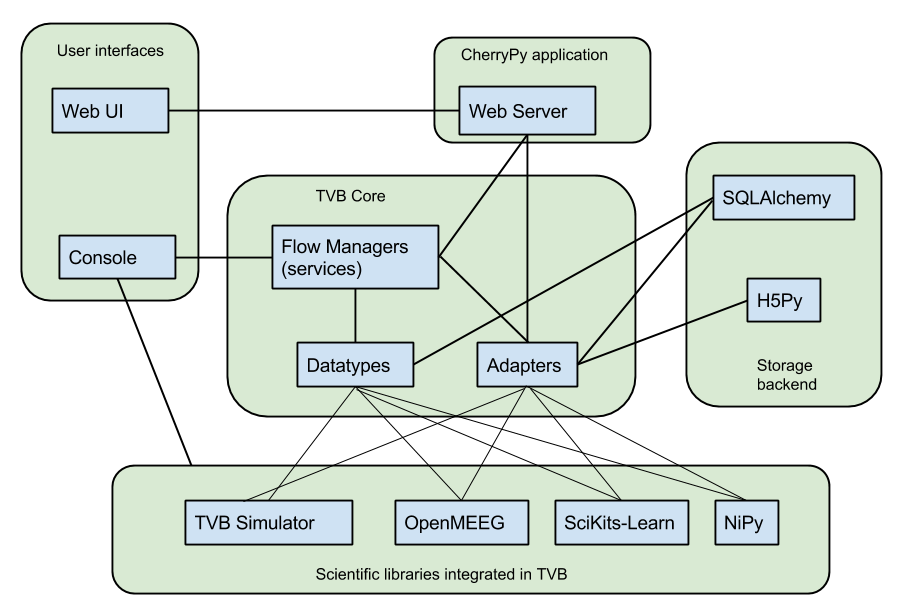
\includegraphics[width=0.7\textwidth]{images/arch.png}
	\caption{\textbf{TVB Architecture} \TVB integrates various scientific 
		libraries through its flexible datatype and adapter abstractions, 
		which allow web and console users to drive work flows in a 
		generic way as well as persistence in a hybrid relation and 
		HDF5 data store.}
	\label{fig:architecture}
\end{figure*}

TVB's architecture, illustrated in Figure \ref{fig:architecture}, was designed 
for the integration of disparate computational
tools, allowing different kinds of data to be managed within one system, and
different routines and processes to work with the kinds of data in the system.
To facilitate this integration, two abstractions have been introduced, around
which the framework is oriented: \textit{datatypes} and \textit{adapters},
serving, briefly, as heavily annotated structs and functions allowing for
programmatic interoperation with the database and generation of and interaction
with the user interface. 

\subsection{Datatypes}

Concretely, a TVB datatype is a Python class with one or more attributes 
that are \textit{trait}s, where a trait specifies both the kind of data
expected for the corresponding attribute, as well additional metadata to
aid in storage and user interface construction. 

During the development of the datatype and traits system, existing implementations
of the concepts of traits were considered, notably Enthought's extensive 
implementation designed to accelerate the design of graphical scientific 
applications and IPython's lighter-weight system designed, to a large extent, 
to provide a robust configuration system. In both cases, the traits are used
to explicitly specify types, allowing runtime values' types to be validated, 
as well as other forms of introspection. This is the case for TVB's traits 
as well, however, Enthought's implementation has significant compiled extensions
(where TVB is intended to be pure-Python); IPython's implementation does not
provide support for arrays, and neither provides integration or mapping to a
database. Lastly, Nipype \citep{gorgolewski2011nipype} provides an approach
specifically targeted toward neuroimaging, but is focused on data processing, 
whereas TVB required database and UI integration.
For these reasons, it was judged useful to develop a system adapted 
to the needs of TVB. 

\begin{lstlisting}[caption={Example of a simple datatype modeling a point in two dimensions}, 
		   label={lst:traitexample}]

class Point2D(MappedType):

    x = Float(label="x",
              doc="horizontal position of point")

    y = Float(label="y",
              doc="vertical position of point")
	      
\end{lstlisting}

Listing \ref{lst:traitexample} shows a datatype modeling a point in two 
dimensions, consisting of two floating point values, \texttt{x} and 
\texttt{y}. This class derives from \texttt{MappedType} whose metaclass, 
before creating the class object, filters attributes for trait instances 
or types and creates a corresponding SQLAlchemy model, which results 
in mapping instances of \texttt{Point2D} to a corresponding table in TVB's
SQL database. The trait base class implements a data descriptor protocol,
i.e. \texttt{\_\_set\_\_} in addition to \texttt{\_\_get\_\_} methods, which, for a
\texttt{MappedType} instance, forwards calls to the get and set methods to 
the corresponding SQLAlchemy method, in turn, interacting with the database.

% trait attribute table
\begin{center}
	\begin{table*}[ht]
		\begin{tabularx}{\textwidth}{lll}
			\toprule
			keyword name & Description  \\
			\midrule
			\texttt{default}          & Default value for current attribute. Will be set on any new instance if not specified otherwise in the constructor.  \\
			\texttt{console\_default} & Define how a default value can be computed for current attribute, when console interface is enabled. \\
			\texttt{range}            & Specify the set of accepted values for current attribute. Mark that this attribute is usable for parameter space exploration. \\
			\texttt{label}            & Short text to be displayed in UI, in front of current attribute. \\
			\texttt{doc}              & Longer description for current attribute. To be displayed in UI as help-text. \\
			\texttt{required}         & Mark current attribute as required for when building a new instance of the parent class. \\
			\texttt{locked}           & When present and \emph{True}, current attribute will be displayed as read-only in the web interface. \\
			\texttt{options}          & Used for attributes of type \emph{Enumerate}, specifying the accepted options as a list of strings. \\
			\texttt{filters\_ui}      & SQL filters on other attributes, to be applied in UI. \\
			\texttt{select\_multiple} & When \emph{True}, current attribute will be displayed as a select with multiple options in UI (default is single-select) \\
			\texttt{order}            & Optional number identifying the index at which current attribute will be displayed in UI. \\
						  & When negative, the attribute is not displayed at all. Ascending order for indices is considered when displaying. \\
			\texttt{use\_storage}     & When \emph{False}, current attribute is not stored in database or file storage. \\
			\texttt{file\_storage}    & Valid values for this attribute are: \emph{None} , \emph{HDF5}, or  \emph{expandable\_HDF5}, \\
						  & When \emph{None}, current attribute is not stored in the file-storage at all. When \emph{HDF5}, we use regular HDF5 file storage. \\
						  & When \emph{expandable\_HDF5} value is set, a HDF5 stored in chunks is used. \\
			\bottomrule
			\end{tabularx}
  	\caption{TVB currently available Traited Attributes}
  	\label{tab:traits}
	\end{table*}
\end{center}

When methods of such a class with annotated attributes are invoked, they may use
the traited attributes directly, accessing either a default value or one given
during the instantiation of the object. Additionally, this allows the web-based
user interface to introspect a class for all of its attributes and their
descriptions, to provide help and choose the proper display form. The explicit
typing also allows such classes to be nearly automatically mapped to storage
tables, providing persistence, when the storage layer is enabled.  Lastly,
because such metadata is used to build the docstring of a class, the console
user also may obtain extensive descriptions of class, attributes, methods and
arguments in the usual way. Table \ref{tab:traits} lists the various parts 
of a traited attribute and how they are used. 

Several trait types are built into TVB's traits system, such as dictionaries,
tuples, lists and arrays, and in most cases, a string representation of the
trait value is stored in the database.  Persisting arrays in SQL, however, is
relatively inefficient, and for this case the data are automatically stored in
HDF5 files. Such options as well as fine-tuning the presentation of different
traits in the user interface are also specified by keyword arguments to the
trait specification.  Table \ref{tab:traits} describes several of these
keywords used throughout the various datatypes in TVB.

In TVB, the datatype classes must typically implement significant functionality
with respect to the user interface, such as filtering instances based on a
user's criterion, as well as scientific methods, such as computing the geodesic
distance on a surface. To facilitate the organization of the code, a base class
declaring the traited attributes is created, followed by two subclasses for 
framework and scientific methods, and a final class that uses the framework and
scientific classes as mixins. The advantage of this scheme is that the domain 
data models can be grouped, and the framework and scientific code may be separated. 

\subsection{Adapters}

The adapter pattern allows arbitrary processes to be invoked by a generic 
framework by detailing the required input data, the outputs, and providing a
method for invoking the process. The input and output data are described in terms of 
TVB's datatypes, which allows processes with different data formats 
to interact as long as an intermediate, common datatype is available. In
TVB, this abstraction extends not only to computational processes such as 
simulation and analysis, but data import, export and, notably visualizations. 

% adapter example
\begin{lstlisting}[caption={Example of a minimal adapter},
                   label={lst:ABCAdapter}]
class DistanceAdapter(ABCAdapter):

  def get_input_tree(self):
      return {'p': Point2D(), 'q': Point2D()}

  def get_output(self):
      return [Float]

  def launch(self, x, y, sqrt=math.sqrt):
      return sqrt((p.x - q.x)**2 + (p.y - q.y)**2)
  	
\end{lstlisting}

Listing \ref{lst:ABCAdapter} presents a minimal example that computes the
distance between two points. Descriptions of the inputs and outputs are
provided by the \texttt{get\_input\_tree} and \texttt{get\_output} methods, and
the computation itself is set off by the \texttt{} method. 
In practice, additional methods are used on adapters to provide for more 
complex initialization and to obtain more information about the space and 
time requirements of the computation. 

This approach scales up to more complex computations, and notably, the
simulator itself is integrated with the web interface through via a
\texttt{SimulatorAdapter}. Additionally, due to the wide-variety of toolboxes available 
for the MATLAB environment, an adapter was created to allow arbitrary code
to be called on any given data type. This adapter works by filling out
a template driver script to handling loading and saving data and launching
the desired code within a try-except clause. This script is with MATLAB or
Octave via a call to the \texttt{os.system} function.

Several alternatives to this approach are possible, such as invoking the MATLAB
engine directly via \texttt{ctypes} and the MATLAB Engine API, or compiling the MATLAB
functions with the MATLAB Compiler. Each, including our approach, has advantages 
and disadvantages. In our case, when configuring TVB, the administrator is asked
to provide the path to the MATLAB or Octave executable, and TVB attempts to 
verify that this executable can be invoked. Beyond this, no other verification 
or protection is currently provided against problematic situations, in part
because we have found it to be sufficiently robust. 

Launching MATLAB can be a relatively slow operation (cold startup ~8 seconds,
cached ~1 second; on a Linux workstation), and where Octave is available, it is
faster (~0.1 seconds). For our use cases, e.g. launching analyses, this works
without problems in a single user situation. In the case that many operations
are necessary, they can be batched into the same script such that MATLAB is
called but once.

One of the uses of this adapter, employs a well-known toolbox for
characterizing anatomical and functional connectivity, the \emph{Brain
Connectivity Toolbox} \citep{Rubinov_2010}.  In TVB, the set of functions,
their inputs and outputs are summarized in an XML file, which is read by a
generic adapter, which handles the data appropriately.

\subsubsection{Analysis \& Visualizers}

TVB does not intend to provide fully featured, complex data analysis
techniques, which have been well covered by other packages. 
Instead, we offer a minimal set of standard algorithms to quickly
validate simulation results or compare with imported patient data; 
these include principal and independent component analyses, 
Fourier and wavelet spectral analyses, correlation and coherence
analyses.

TVB visualizers employ different techniques, depending on the nature of
the data to display and degree of interactivity required, including WebGL,
D3.js generated SVG, Matplotlib's HTML5 Canvas backend, as well as other
HTML5 Canvas Javascript libraries for simpler, static graphs. In each case,
an adapter is developed to abstract over the differences between these
techniques, allowing the framework to treat it without knowing the details.

Interaction-intensive tools that combine several techniques have been developed
for specific purposes, for example working with connectivity matrices, 
configuring the phase space structure of the mass model, or designing
spatiotemporal stimuli. These are built upon the same abstractions and have been
detailed in the general overview of TVB \citep{Sanz-Leon_2013}.

\section{Simulator}

% into
A significant part of TVB is simulating large-scale brain networks. While
several existing simulators could have been adapted, we have estimated that
TVB style simulations are far enough outside the design of other simulators to
make a new development necessary. We discuss these reasons in the following. 

% existing
Existing neural network simulators typically focus either on abstract rate neurons, 
modelling neurocognitive processes, or 
multicompartmental neurons treating complex spatial
geometries, e.g. NEURON \citep{Hines_2001}, modelling the interaction of 
channel distributions in dendrites.  More recently, due to interest in
the computational properties of spiking neurons and their relevance to
experimental observations, simulators designed for spiking or oscillating neurons
have become prominent, including Brian \citep{Goodman_2009}, which we initially 
considered for our simulations.
In TVB the network is defined with neural mass or field
models \citep{Deco_2008a, Coombes_2010} rather than cellular models. The
spatial extent of the modeled dynamics is macroscopic and scales reasonably 
to the entire cortex, and uses empirical measurements of cortico-cortical
connectivity. Several technical issues are unique to this scale, such
as efficient handling of dense $N^2$ inter-regional delays and integration
of neural field-like models and connectivity on triangular meshes in 3D.
Finally, comparison with experimental data requires forward solutions
that transform physiological signals to the commonly
used imaging modalities such as EEG, MEG and fMRI.
For these reasons, TVB required a new simulator, built around the paradigm
of whole-brain scale simulation.

The simulator in TVB resembles popular neural network simulators in 
many fundamental ways, both mathematically and in terms of informatics 
structures, however we have found it necessary to introduce auxiliary
concepts particularly useful in the modeling of large scale brain 
networks. In the following, we will highlight some of the interesting
principles and capabilities of TVB's simulator and give rough characterization
of the execution time and memory required in typical simulations.

\subsection{Node dynamics}

In TVB, nodes are not considered to be abstract neurons nor necessarily small
groups thereof, but rather large populations of neurons. Concretely, the main
assumption of the neural mass modeling approach in TVB is that large pools of
neurons on the millimeter scale are strongly approximated by population level
equations describing the major statistical modes of neural dynamics
\citep{Freeman_1975book}. Such an approach is certainly not new; one of the
early examples of this approach consist of the well known Wilson-Cowan
equations \citep{Wilson_1973}. Nevertheless, there are important differences in
the assumptions and goals from modeling of individual neurons, where the goal
may be to reproduce correct spike timing or predict the effect of  a specific
neurotransmitter. A second difference lies in coupling: chemical coupling is
often assumed to be pulsatile, or discrete, between neurons, whereas for
mesoscopic models it is considered continuous. Typically the goal of neural
mass modeling is to study the dynamics that emerge from the interaction of two
or more neural masses and the network conditions required for stability of a
particular spatiotemporal pattern. In the following, we shall  briefly discuss
some of the models available in TVB.

This modeling paradigm may be contrasted with population density models modelling the
dynamics of large populations of neurons
(\cite{de1993stochastical, omurtag2000simulation, knight2000dynamics,
gerstner2000population}; see \cite{Deco_2008a} for a review).  The large number
of neurons impart the state space with a probability density, and population
density methods describe the evolution of this density via the Fokker-Planck
(FP) equation \citep{risken1996fokker} comprised of flow and dispersion terms.
This approach assumes that the afferents on neurons in one population are
uncorrelated.  Neural mass models, from this paradigm, are obtained as a
special case when the full ensemble density dynamics is replaced by a mass at
one point in state space and its dynamics summarize the movement of density in
state space, losing information on the changes in shape of the density.  In the
full, nonlinear FP form, different density moments can couple, even within and
between populations, meaning the membrane potential variance of one population
could affect the average of another. Neural mass models ignore this possibility
by coupling only the first moments, though this may be overcome by e.g.
extending mass models with more than one mode \citep{Stefanescu_2008,
Stefanescu_2011}.  TVB does not implement density methods via the FP equation
because the additional moments required to derive physiologically relevant
variables (such as LFP or firing rate), would add an additional level of
complexity.  

In TVB, many neural mass models from the literature are available, including
the often used Jansen-Rit model of rhythms and evoked responses arising from
coupled cortical columns \citep{Zetterberg_1978, Jansen_1995,Spiegler_2010}.
\citeauthor{David_2003}'s slightly modified form has been extensively applied
within a Bayesian framework known as Dynamic Causal Modeling (DCM) for modeling
neuroimaging data via estimation of biophysical parameters of underlying
network models \citep{David_2003, friston2003dynamic, david2006dynamic}.  The
Jansen-Rit model is a biophysical one, whose state variables and parameters are
readily interpretable with respect to experiments, however it has at least six
state equations involving several exponential expressions. For cases where it
is desirable to have a simpler and more performant model, a generic
two-dimensional oscillator model is also provided by TVB (see 
\cite{strogatz2001nonlinear} and \cite{guckenheimer1983nonlinear} for 
for generic mathematical references on two-dimensional dynamical systems).
This model produces
damped, spike-like or sinusoidal oscillations, which, in the context of a
network, permit the study of network phenomena, such as synchronization of
rhythms or propagation of evoked potentials.  Other models implemented in TVB
include the Wilson-Cowan description of functional dynamics of neural tissue
\citep{Wilson_1972}, the Kuramoto model describing synchronization
\citep{Kuramoto_1975, Cabral_2011}, two and three dimensional statistical
mode-level models describing populations with excitability distributions
\citep{Stefanescu_2011, Stefanescu_2008}, a reduction of
\citeauthor{Wong_2006}'s (\citeyear{Wong_2006}) model as presented by
\cite{Deco_2013} and a lumped version of Liley's model \citep{Liley_1999,
Steyn-Ross_1999}.  Lastly, adding a model only requires subclassing a base
\texttt{Model} class and providing a  \texttt{dfun} method to compute the right
hand sides of the differential equations. 

\subsection{Network structure}

The network of neural masses in TVB simulations directly follows from  two
 geometrical constraints on cortical dynamics. The first is the
large-scale white matter fibers that form a non-local and heterogeneous
(translation variant) connectivity, either measured by anatomical tracing
(CoCoMac, \cite{Koetter_2004}) or diffusion-weighted imaging 
\citep{Hagmann_2008, Honey_2009, Bastiani_2012}.
The second is that of horizontal projections
along the surface, which are often modeled with a translation invariant
connectivity kernel, approximating a neural field (however, as with other
parameters in the simulator, connectivity kernel parameters that vary 
across space can also be used).

TVB does not assume that the network structure is constant during the
simulation, but does not currently implement the modeling of structural
modulation. This can however be added during simulation.

\subsubsection{Large-scale connectivity}

The large-scale region level connectivity at the scale of centimeters,
resembles more a traditional neural network than a neural field, in that,
neural space is discrete,  each node corresponding to a neuroanatomical
region of interest, such as V1, etc. It is at this level that inter-regional 
time delays play a large role, whereas the time delays due to 
lateral, local projections are subsumed under the dynamics of the node.

It is often seen in the literature that the inter-node coupling functions
\textit{are} part of the node model itself. In TVB, we have instead 
chosen to factor such models into the intrinsic neural mass dynamics, where each 
neural mass's equations specify how connectivity contributes to the
node dynamics, and the coupling function, which specifies how the activity
from each region is mapped through the connectivity matrix. Common coupling 
functions are provided such as the linear, difference and periodic functions
often used in the literature.

\subsubsection{Local connectivity}

The local connectivity of the cortex at the scale of millimeters provides
a continuous 2D surface along horizontal projections connecting
cortical columns. Such a structure has previously been modeled by
neural fields \citep{Amari_1977, Jirsa1996, Jirsa_1997, Liley_1999}. 
In TVB, surface meshes provide the spatial discretization of neural anatomy. A
neural mass is placed on each vertex, and the geodesic distances between each
mass is computed. A local connectivity kernel assigns, for each distance, a
connection weight between masses. This kernel is usually chosen such that it
decays exponentially with distance.
The associated sampling problem has been studied in detail by \citep{Spiegler_2013},
which finds the approximation to be reasonable, depending on the properties
of the mesh and the imaging modalities that sample the activity simulated
on the mesh. In fact,
the implementation of the local connectivity kernel is such
that is can be re-purposed as a discrete Laplace-Beltrami operator,
allowing for the implementation of true neural field models that 
use a second-order spatial derivative as their explicit spatial term.

TVB currently provides several connectivity kernels, of which a Gaussian
is one commonly used. Once a cortical surface mesh 
and connectivity kernel and its parameters are chosen, the geodesic
distance (i.e. the distance along the cortical surface) is evaluated
between all neural masses \citep{Mitchell1987}, and a cutoff is chosen
past which the kernel falls to 0. This results in a sparse matrix that 
is used during integration to implement the approximate neural field. 

\subsection{Integration of stochastic delay differential equations}

In order to obtain numerical approximations of the network model 
described above, TVB provides both deterministic and stochastic
Euler and Heun integrators,
following standard numerical solutions to stochastic
differential equations \citep{Kloeden_1995,Mannella_2002,Mannella_1989}.

While the literature on numerical treatment of delayed or 
stochastic systems exists, it is less well known how to treat 
the presence of both. For the moment, the methods implemented by TVB
treat stochastic integration separately from delays. 
This separation coincides with a modeling assumption that in
TVB the dynamical phenomena to be studied are largely determined
by the interaction of the network structure and neural mass dynamics, 
and that stochastic fluctuations do not fundamentally reorganize the
solutions of the system \citep{Ghosh_2008,Deco_2009,Deco_2011,Deco_Senden_2012}.

Due to such a separation, the implementation of delays in the
regional coupling is performed outside the integration step,
by indexing a circular buffer containing the recent simulation 
history, and providing a matrix of delayed state data to the 
network of neural masses. While the number of pairwise
connections rises with $n_{region}^2$, where $n_{region}$ is
the number of regions in the large-scale connectivity, 
a single buffer is used, with a shape
$(horizon, n_{cvar}, n_{region})$ where $horizon = max(delay) + 1$,
and
$n_{cvar}$ is the number of coupling variables. Such a scheme helps 
lower the memory requirements of integrating the delay equations.

\subsection{Forward solutions}

TVB provides forward solutions to generate neuroimaging data from 
simulated neural activity based on biophysical models 
\citep{Buxton_2004, Jirsa_2002}. Practically, it is also often
necessary to simply reduce the size of data, especially in the case of 
surface simulations. TVB implements these two functionalities in
a set of classes called \texttt{Monitors}, each of which receives
the raw simulation output and applies a spatial, temporal or spatiotemporal
kernel to the output to obtain the simulation output passed to the
user or stored. 

Where necessary, monitors employ more than one internal buffer. In the case of 
the fMRI monitor, a typical sampling frequency of simulation may be upward of 
64 kHz, and the haemodynamic response function may last several seconds, 
using only a single buffer could require several gigabytes of memory for the 
fMRI monitor alone. Given that 
the time-scale of simulation and fMRI differ by several orders of magnitude, 
the subsequent averaging and downsampling is justified. 

In the cases of the EEG and MEG monitors, the temporal kernel implements a
simple temporal average, and the spatial kernel consists of a so-called
lead-field matrix as typically derived from a combination of structural imaging
data, providing the locations and orientations of the neural sources and the
locations and orientations of the EEG electrodes and MEG gradiometers and
magnetometers.  As the development and implementation of such lead-fields is
well developed elsewhere
\citep{Sarvas_1987,Hamalainen_1989,Jirsa_2002,Nolte2003,Gramfort_2010}, TVB
provides access to the well-known OpenMEEG package.

\subsection{Parameter sweeps}

As is often the case in modeling, there are several or many parameters of the
simulation that may be relevant, and to facilitate the exploration of the effects
of variation of parameters, the user, from the web interface, can select one or
two parameters and create a grid of simulations that are run in parallel on the
computer. Afterwards, a summary visualization of the simulations is displayed. For
example, this simple approach can be useful to find the parameter
values within a range nearest to a bifurcation from a fixed point to a limit
cycle: to each resulting time series, the global variance is computed, and 
displayed as a function of parameter values. 

Nevertheless, no tools are provided to perform correct estimation or fitting
of the models, and this is not currently a goal for TVB. 

For this purpose, as well as more sophisticated explorations of the parameter
space it may be useful to turn to scripting the simulator in Python, and pulling
in functionality from other libraries.

\subsection{Performance}

A priority of the simulator in TVB is to attain a high level of performance
while remaining in pure Python. In order to see where the simulator 
spends most of its time, we have profiled 
a set of eight characteristic simulations
%on both memory use, specifically the heap size as measured by Valgrind's 
%\texttt{massif} tool \citep{nethercote2007valgrind}, 
on function timing as measured by the 
\texttt{cProfile} module of the standard library. 

Measurements were
performed on an HP Z420 workstation, with a single Xeon E5-1650
six-core CPU running at 3.20 GHz, L1-3 cache sizes 384 KB, 1536 KB
and 12 MB respectively, with main memory 4 x 4 GB DDR3 at 1600 Mhz,
running Debian 7.0, with Linux kernel version 3.2.0-4-amd64. 
The 64-bit Anaconda Python distribution was used with additional Accelerate
package which provides acceleration of common routines based on the 
Intel Math Kernel Library. A Git checkout of the trunk branch of TVB 
was used with SHA \texttt{6c644ab3b5}.

Eight different simulations were performed corresponding to the combinations of
either the generic 2D oscillator or Jansen-Rit model, region-only
or use of cortical surface, and two conduction speeds, $v_c = 2.0$ and
$v_c = 20.0$ (m/s). In each case, a temporal average monitors at 512 Hz
is used, and the results are discarded. The region-only simulation was
run for one second while the surface simulation was run for 100 ms. 

	% profiling table
	\begin{table}
	{\footnotesize \begin{tabular}{r | r | l }
	Sim. &        Time (s) &                     Module/Function \\
	\hline \\
	R / G2D / 20  &         11.72 & \texttt{<numpy.core.multiarray.array>} \\
	&          6.14 & \texttt{numpy.lib.npyio}, \texttt{loadtxt} \\
	 &         5.18 & \texttt{tvb.simulator.simulator}, \texttt{\_\_call\_\_} \\
	 &         3.18 & \texttt{numpy.lib.npyio}, \texttt{pack\_items} \\
	 &          2.56 & \texttt{numexpr.necompiler}, \texttt{evaluate} \\
	\hline
	2 &         11.87 & \texttt{<numpy.core.multiarray.array>} \\
	&         6.10 & \texttt{numpy.lib.npyio}, \texttt{loadtxt} \\
	 &         5.54 & \texttt{tvb.simulator.simulator}, \texttt{\_\_call\_\_} \\
	 &         3.16 & \texttt{numpy.lib.npyio}, \texttt{pack\_items} \\
	 &         2.50 & \texttt{numexpr.necompiler}, \texttt{evaluate} \\
	\hline
	 JR / 20  &         14.21 & \texttt{<numpy.core.multiarray.array>} \\
	&         9.99 & \texttt{tvb.simulator.simulator}, \texttt{\_\_call\_\_} \\
	 &         7.28 & \texttt{tvb.simulator.models}, \texttt{dfun} \\
	 &           6.20 & \texttt{numpy.lib.npyio}, \texttt{loadtxt} \\
	 &         3.24 & \texttt{numpy.lib.npyio}, \texttt{pack\_items} \\
	\hline
	2 &         14.21& \texttt{<numpy.core.multiarray.array>} \\
	&         10.57& \texttt{tvb.simulator.simulator}, \texttt{\_\_call\_\_} \\
	 &         7.40& \texttt{tvb.simulator.models}, \texttt{dfun} \\
	 &         6.12& \texttt{numpy.lib.npyio}, \texttt{loadtxt} \\
	 &         3.25& \texttt{numpy.lib.npyio}, \texttt{pack\_items} \\
	\hline
	S / G2D / 20 &         126.61& \texttt{<\_csc.csc\_matvec>} \\
	&         57.56& \texttt{<numpy.core.multiarray.array>} \\
	 &         56.17& \texttt{<gdist.local\_gdist\_matrix>} \\
	 &           9.05& \texttt{<numpy.core.\_dotblas.dot>} \\
	 &         7.56& \texttt{numpy.lib.npyio}, \texttt{loadtxt} \\
	\hline
	2 &         125.95& \texttt{<\_csc.csc\_matvec>} \\
	&         57.75& \texttt{<numpy.core.multiarray.array>} \\
	 &         56.16& \texttt{<gdist.local\_gdist\_matrix>} \\
	 &         12.10& \texttt{<numpy.core.\_dotblas.dot>} \\
	 &         7.37& \texttt{numpy.lib.npyio}, \texttt{loadtxt} \\
	\hline
	JR / 20 &         126.31& \texttt{<numpy.core.multiarray.array>} \\
	&         56.37& \texttt{<gdist.local\_gdist\_matrix>} \\
	 &         19.52& \texttt{<numpy.core.\_dotblas.dot>} \\
	 &         9.47& \texttt{tvb.simulator.models}, \texttt{dfun} \\
	 &         8.87& \texttt{<mtrand.RandomState.normal>} \\
	\hline
	2 &         126.09& \texttt{<numpy.core.multiarray.array>} \\
	&         56.79& \texttt{<gdist.local\_gdist\_matrix>} \\
	 &          29.10& \texttt{<numpy.core.\_dotblas.dot>} \\
	 &         14.18& \texttt{<mtrand.RandomState.normal>} \\
	 &         9.57& \texttt{tvb.simulator.models}, \texttt{dfun} \\
	\hline

	\end{tabular}}
	\caption{Profiling results for several simulation types, ``R'' for region 
	level simulations, ``S'' for surface level. ``G2D'' signifies the generic
	two-dimensional oscillator whereas ``JR'' is the Jansen-Rit model. Finally,
	either 20 m/s or 2 m/s conduction velocity was used. Time is given as the
	total time spent in the method or function listed in the right column.}
	\label{tab:profiling}
	\end{table}


As can be seen in Table \ref{tab:profiling},
significant time is spent on array manipulations written in C (marked by those
function names surrounded by angle brackets), from the NumPy and SciPy libraries, 
including the spare matrix-vector multiplication used to compute the local connectivity.
In some cases, such as the 
neural mass model definitions, large expressions implicitly generate many 
temporary arrays, which can be ameliorated by using the \texttt{numexpr} module
to compute the expressions element-wise: TVB's \texttt{JansenRit} model is
implemented as regular Python expressions of NumPy arrays, while a subclass
\texttt{JRFast} uses \texttt{numexpr.evaluate}, resulting in a 40 \% improvement
in overall runtime.

Given that the numerical routines are written in Python to maintain a high level
of flexibility, it is expected that there are limits on the performance, especially 
compared to compiled languages. Ongoing work on the simulator will take advantage of
newer programming paradigms and hardware, such as OpenCL and graphics processing units; 
this sort of programming is facilitated by Python libraries such as PyOpenCL
\citep{klockner2012pycuda}.

\section{Discussion}

In this article, we have described several informatics aspects of the
implementation of a integrative platform for modeling neuroimaging data.
Despite the currently available functionality in TVB, in the following we wish
to make several points about its context as a modeling tool as well as 
future work. 

\subsection{Modelling goals}

The literature on network models frequently presents work in which a model
is constructed in order to estimate structure and parameters from 
experimental data, and the DCM framework has significantly advanced 
methods for such estimations for both fMRI and M/EEG data. Indeed, there
are similarities in the underlying mathematical machinery between DCM and 
TVB. However, the estimation of parameters in the case of TVB's models
is still a challenging question and for now is not a goal of the framework. 
For this reason, none of the requisite estimation tools are currently 
provided by TVB.

Related to the goal of estimating model parameters for brain network models
is the modeling of function or functional dynamics itself 
\citep{erlhagen2002dynamic, eliasmith2012large}. TVB allows a user
to fully specify the node dynamics and connectivity, yet no support
is currently providing for deriving a set of parameters that leads to 
a particular functional state. This, like the estimation problem, is 
an open question, particularly for models as complex as those simulated 
within TVB.

\subsection{Future work}

Since the recent release of the $1.0$ version of TVB, it has been 
officially considered \textit{feature} complete, however, in several
cases, the development of features has outstripped documentation 
and testing. Going forward, general priorities include
advancing test coverage, improving documentation for users, and
preparing PyPI and Debian packages. In the mean
time, TVB's Google groups mailing list continues to
provide an open forum for troubleshooting and sharing of user experiences.

While several mathematical challenges are presented by the TVB models, 
one of the bottlenecks is the speed of the numerical simulation.
To address this, continued optimization of C and GPU code generation
will take place, e.g. to perform parallel parameter sweeps. 

Additionally, an interface \textit{from} MATLAB to TVB 
is being developed to allow use of the simulator through a simple
set of MATLAB functions. As this infrastructure is based on an HTTP and 
JSON API, it will likely enable other applications to work with TVB as well.

Lastly, as TVB was originally motivated to allow a user to move from acquired
data to simulated data as easily as possible, we will continue to integrate
several of the requisite steps that are not currently covered, such as analysis
of DSI data to produce connectivity matrices, though in many cases, such as
parcellation and labeling of cortical areas, these steps may continue to
require interaction with other software. Altogether, TVB provides a
rich platform for integrating neuroinformatics tools with an emphasis on
analysis and modeling of human neuroimaging data.


\section*{Acknowledgments}
Several authors have also participated in the
development of TVB. They are listed in the \texttt{AUTHORS} file 
of the source code and deserve our warm acknowledgments. LP wishes to thank
specifically Y.~Mahnoun for his role in the design and development
of the first prototype of the TVB architecture. 

The authors wish to thank two anonymous reviewers for their constructive comments
and questions.

The research reported herein
was supported by the  Brain Network Recovery Group through the James S.
McDonnell Foundation and the FP7-ICT BrainScales. PSL and MMW received
support by from the French Minist\`{e}re de Recherche and the Fondation
de Recherche Medicale.

\bibliographystyle{apalike}
\bibliography{bib}

\end{document}

